\begin{frame}{Notation}
    $(\Fs, \Hs) =
    \begin{cases}
        f_1(x_1, \dots, x_n) = 0 \\
        f_2(x_1, \dots, x_n) = 0 \\
        \dots \\
        f_a(x_1, \dots, x_n) = 0 \\
        \hline
        h_1(x_1, \dots, x_n) > 0 \\
        h_2(x_1, \dots, x_n) > 0 \\
        \dots \\
        h_s(x_1, \dots, x_n) > 0 \\
    \end{cases}
    $

    \pause

    \begin{block}{Range axiom $R_i$ for a variable $x_i$:}
        \begin{itemize}
            \item $\mathbf{\{0, 1\}}$ basis: $x_i^2 - x_i$;
            \item $\mathbf{\{\pm 1\}}$ basis: $x_i^2 - 1$.
        \end{itemize}
    \end{block}

   
\end{frame}


\begin{frame}{Proof Systems}

    The \deftext{Sum-of-Squares} ($\SOS$) proof of $(\Fs, \Hs)$:
    $$
        \sum_{u = 1}^{a} p_u f_u + \sum_{j = 1}^{n} r_j R_j + \sum_{v = 1}^{b} q_v^2 h_v = -1
    $$
    $f_u \in \Fs, h_v \in \Hs \cup {1}$

    \pause
    \vspace{0.4cm}

    The \deftext{Polynomial Calculus} ($\PCR[\field]$) proof of $\Fs$ is a sequence
    $(p_1, p_2, p_3, \dots, p_{\ell})$:
    \pause
    \begin{itemize}
        \item $p_i \in \Fs \cup \bigcup\limits_{j = 1}^{n} \{R_j\}$;
        \pause
        \item $p_i = x_j p_k$ for some $j$ and $k < i$;
        \pause    
        \item $p_i = \alpha p_k + \beta p_s$ for some $k, s < i$ and $\alpha, \beta \in \field$;
        \pause
            \item $p_{\ell} = 1$.
    \end{itemize}

    \pause
    \vspace{-0.2cm}
    \begin{minipage}{0.4\linewidth}
        $\Fs =
        \begin{cases}
            xy - 1 = 0 \\
            yz + 1 = 0 \\
            x + z - 2 = 0
        \end{cases}$
    \end{minipage}
    \pause
    \begin{minipage}{0.58\linewidth}
        \begin{prooftree}
            \AxiomC{$x + z - 2$}
            \UnaryInfC{$x y + y z - 2y$}
            \AxiomC{$xy - 1$}
            \AxiomC{$yz + 1$}
            \BinaryInfC{$xy + yz$}
            \BinaryInfC{$2y$}
            \UnaryInfC{$2 y^2$}
            \AxiomC{$y^2 - 1$}
            \BinaryInfC{$1$}
        \end{prooftree}
    \end{minipage}



\end{frame}


\begin{frame}{Hierarchy}

    \tikzset{
    >=latex,
    perpinterface/.style = {
        postaction = {
            draw,
            decorate,
            decoration = {
                ticks,
                raise = 0.07cm,
                amplitude = 0.07cm,
                segment length = 1mm
            }
        }
    },
    % пружина
    vert/.style = {
        draw,
        ellipse
    },
    tikzart-fire/.pic = {
        \draw[fill = red!60] (0, 0) .. controls (0.3, 0) and (0.6, 0.1) .. (0.7, 0.3)
            .. controls (0.8, 0.5) and (0.85, 0.6) .. (0.8, 0.9)
            .. controls (0.75, 1.1) and (0.7, 1.2) .. (0.6, 1.4)
            .. controls (0.65, 1.2) and (0.6, 1.05) .. (0.5, 0.9)
            .. controls (0.5, 1.2) and (0.2, 1.3) .. (0.1, 1.6)
            .. controls (0.05, 1.75) and (0.1, 2) .. (0.2, 2.1)
            .. controls (-0.1, 2) and (-0.2, 1.85) .. (-0.3, 1.7)
            .. controls (-0.4, 1.5) and (-0.45, 1.3) .. (-0.4, 1.1)
            .. controls (-0.5, 1.2) and (-0.51, 1.4) .. (-0.5, 1.5)
            .. controls (-0.75, 1.2) and (-0.8, 0.7) .. (-0.7, 0.5)
            .. controls (-0.6, 0.28) and (-0.4, 0) .. (0, 0);
            \fill[white] (0, 0) .. controls (0.3, 0) and (0.52, 0.34) .. (0.37, 0.61)
            .. controls (0.4, 0.54) and (0.32, 0.32) .. (0.25, 0.25)
            .. controls (0.3, 0.35) and (0.25, 0.5) .. (0.2, 0.6)
            .. controls (0.1, 0.8) and (-0.05, 1) .. (0, 1.2)
            .. controls (-0.32, 1) and (-0.3, 0.72) .. (-0.2, 0.47)
            .. controls (-0.3, 0.51) and (-0.31, 0.6) .. (-0.33, 0.7)
            .. controls (-0.4, 0.6) and (-0.4, 0.5) .. (-0.4, 0.4)
            .. controls (-0.35, 0.18) and (-0.2, 0) .. (0, 0);
    }
}


    
\begin{tikzpicture}
    \node[vert] (res) at (1, 0) {$\Res$};
    \node[vert] (ns) at (-3, 0) {$\NS$};
    \node[vert] (cp) at (3, 1) {$\CP$};
    \node[vert] (acf) at (1.2, 1.5) {$\AC_0$-Frege};
    \node[vert] (resl) at (-1, 2.1) {$\ResL$};
    \node[vert] (acfp) at (0.5, 3.5) {$\AC_0[p]$-Frege};
    \node[vert] (fre) at (0.5, 5) {Frege};
    \node[vert] (ips) at (-2, 6) {$\PrSys{IPS}$};
    \node[vert] (pcr) at (-3, 2) {$\PCR[]$};
    \node[vert] (sos) at (-4, 2.5) {$\SOS$};

    \node[vert] (ns2) at (-5.5, 0) {$\NS_{\{\pm 1\}}$};
    \node[vert] (pcr2) at (-6, 2) {$\PCR[]_{\{\pm 1\}}$};
    \node[vert] (sos2) at (-6.8, 3) {$\SOS_{\{\pm 1\}}$};

    \node[vert] (cps) at (-4, 6.5) {$\PrSys{CPS}$};

    \draw[->] (res) -- (cp);
    \draw[->] (cp) to[out = 90, in = -20] (fre);
    \draw[->] (res) -- (resl);
    \draw[->] (res) -- (acf);
    \draw[->] (res) -- (pcr);
    \draw[->] (ns) -- (pcr);
    \draw[->] (resl) -- (acfp);
    \draw[->] (acf) -- (acfp);
    \draw[->] (acfp) -- (fre);
    \draw[->] (fre) -- (ips);
    \draw[->] (ips) -- (cps);

    \draw[->] (pcr) -- (ips);
    \draw[->] (sos) -- (cps);

    \draw[->] (ns2) -- (pcr2);
    \draw[->] (pcr2) -- (ips);
    \draw[->] (sos2) -- (cps);

    \node[inner sep = 0pt] at (-7, 5.5)
    {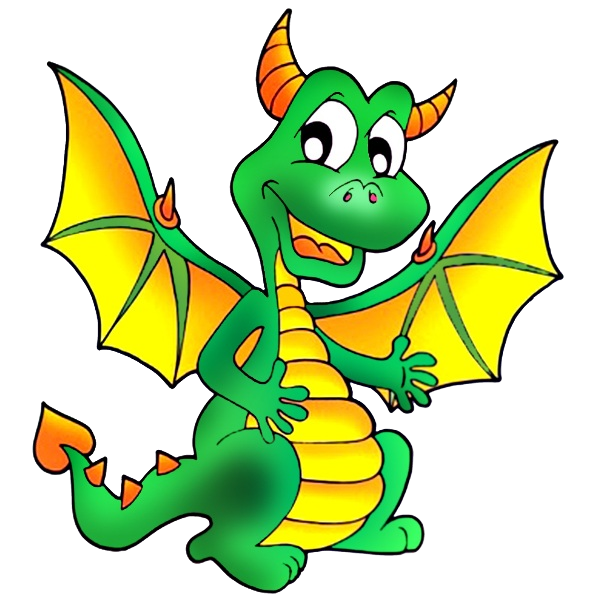
\includegraphics[width = .2\textwidth]{pics/dragon.png}};

    \pause
    \draw[ultra thick, blue] (-4, -1) to[out = 110, in = 230] (-4.4, 3) to[out = 50, in = 180] (3.5, 1.8);
    \foreach \point in {(1.5, 3), (-2, 4), (-6, 1)}{
        \pic at \point {tikzart-fire};
    }
    
\end{tikzpicture}
    
\end{frame}



\begin{frame}{Results}

    $d_0$ is the degree of $(\Fs, \Hs)$. $n$ is the number of variables of $(\Fs, \Hs)$.
    
    \begin{theorem}
        Any $\SOSf$-proof of $(\Fs, \Hs) \circ \MAJ(z_1, z_2, z_3)$ has size
        $\exp(\Omega(\frac{(d - d_0)^2}{n}))$. There $d$ is an $\SOS$-degree of $(\Fs, \Hs)$.
    \end{theorem}

    \pause

    \begin{theorem}
        If $\varphi$ is a random $11$-CNF formula then whp any $\SOSf$-proof or $\PCRf[\field]$-proof of
        $\varphi$ has size $\exp(\Omega(n))$.
    \end{theorem}

    \pause
    \begin{theorem}
        Any $\PCRf[\field]$-proof of Pigeonhole Principle has size $\exp(\Omega(n))$.
    \end{theorem}

    $\SOSf$ is strictly stronger than $\PCRf[\mathbb{R}]$.

\end{frame}